\chapter{Diseño e Implementación} % Main chapter title

\label{Chapter3} % Change X to a consecutive number; for referencing this chapter elsewhere, use \ref{ChapterX}
\definecolor{mygreen}{rgb}{0,0.6,0}
\definecolor{mygray}{rgb}{0.5,0.5,0.5}
\definecolor{mymauve}{rgb}{0.58,0,0.82}

%----------------------------------------------------------------------------------------

La idea de este capítulo es explicar los criterios utilizados en el desarrollo del producto y justificar las decisiones de diseño; así como también explicar el detalle de la implementación de los distintos aspectos del producto.

\section{Hardware}
\label{section:hardware}

En el contexto del presente trabajo, se desarrolló un prototipo funcional del producto final. Este prototipo presenta las mismas funciones que el equipo final pero no se ajusta a los lineamientos estéticos y mecánicos que si deberá cumplir el producto. Es por esto que el prototipo diseñado tiene dimensiones mucho más grandes que las que tendrá, lo cual facilitó las mediciones y pruebas que se debieron realizar para comprobar el correcto funcionamiento tanto del hardware como del firmware. 

En la Figura \ref{fig:prototipo} puede verse una fotografía del prototipo. En la misma se puede apreciar el PCB diseñado y las dos conexiones principales: a la izquierda del gabinete la conexión a la línea eléctrica y a la derecha la conexión a la carga eléctrica. La placa fue colocada dentro de un gabinete que por supuesto no tiene relación alguna con el gabinete que finalmente se utilizará. Simplemente cumple la función de facilitar la manipulación del prototipo.

\begin{figure}[h]
	\centering
	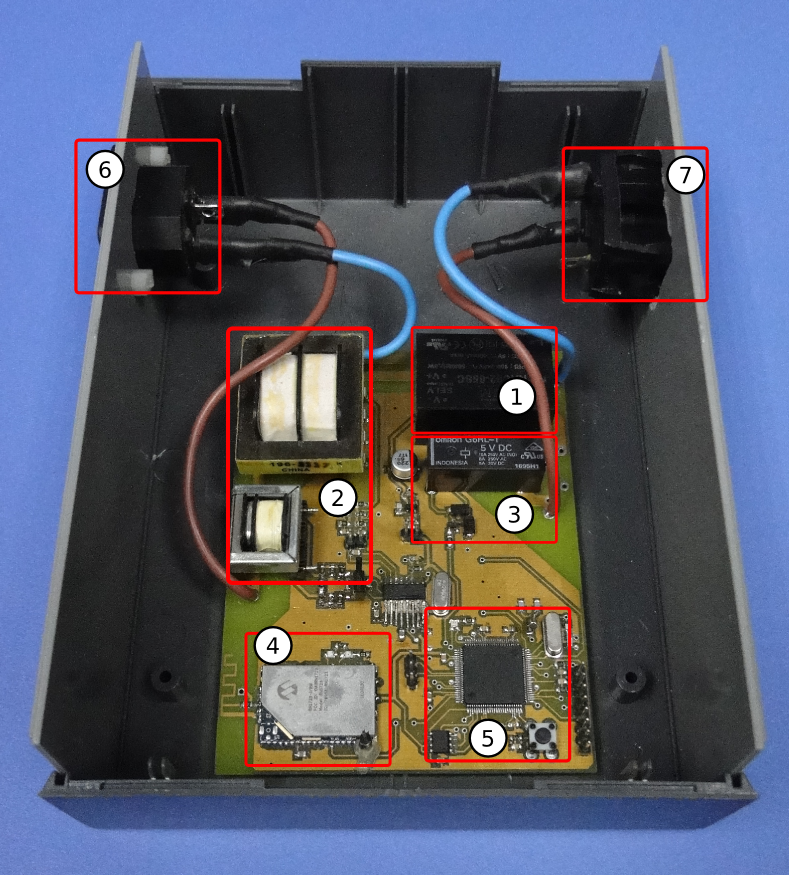
\includegraphics[width=11cm]{./Figures/3_1_prototipo_1.png}
	\caption{Prototipo funcional del Smart Plug. 1 - Fuente de alimentación. 2 - Adaptación de las señales de línea. 3 - Control de la carga. 4 - Módulo WiFi. 5 - Microcontrolador, led bicolor, pulsador y memoria EEPROM. 6 - Conexión a la línea eléctrica. 7 - Conexión a la carga.}
	\label{fig:prototipo}
\end{figure}

Los bloques mencionados en la Figura \ref{fig:prototipo} son explicados en las Subsecciones \ref{subsec:esquematico_general} y \ref{subsec:detalles_hardware}.

A pesar de ser un prototipo funcional, el hardware se diseño pensando en las caracteríticas finales que tendrá el producto. Por lo tanto se debieron definir las especificaciones deseadas para el equipo:

\begin{itemize}
\item Tensión máxima de operación: 240VAC
\item Corriente máxima de operación: 5A
\end{itemize}

Para una tensión de operación de 220VAC, la máxima potencia que se puede conectar es de 1100W. Para un primer producto se buscó cubrir la automatización de aparatos eléctricos de baja potencia como lámparas, ventiladores, electrodomésticos pequeños, televisores, etc. El manejo de equipos de mayor potencia como aires acondicionados, estufas eléctricas, hornos eléctricos, etc, será cubierto en un futuro cuando se modifique el hardware para soportar una mayor corriente, generando así un nuevo producto.



\subsection{Esquemático general}
\label{subsec:esquematico_general}

En la Figura \ref{fig:hardware_diagrama_bloques} pueden verse los principales bloques funcionales del prototipo.

\begin{figure}[h]
	\centering
	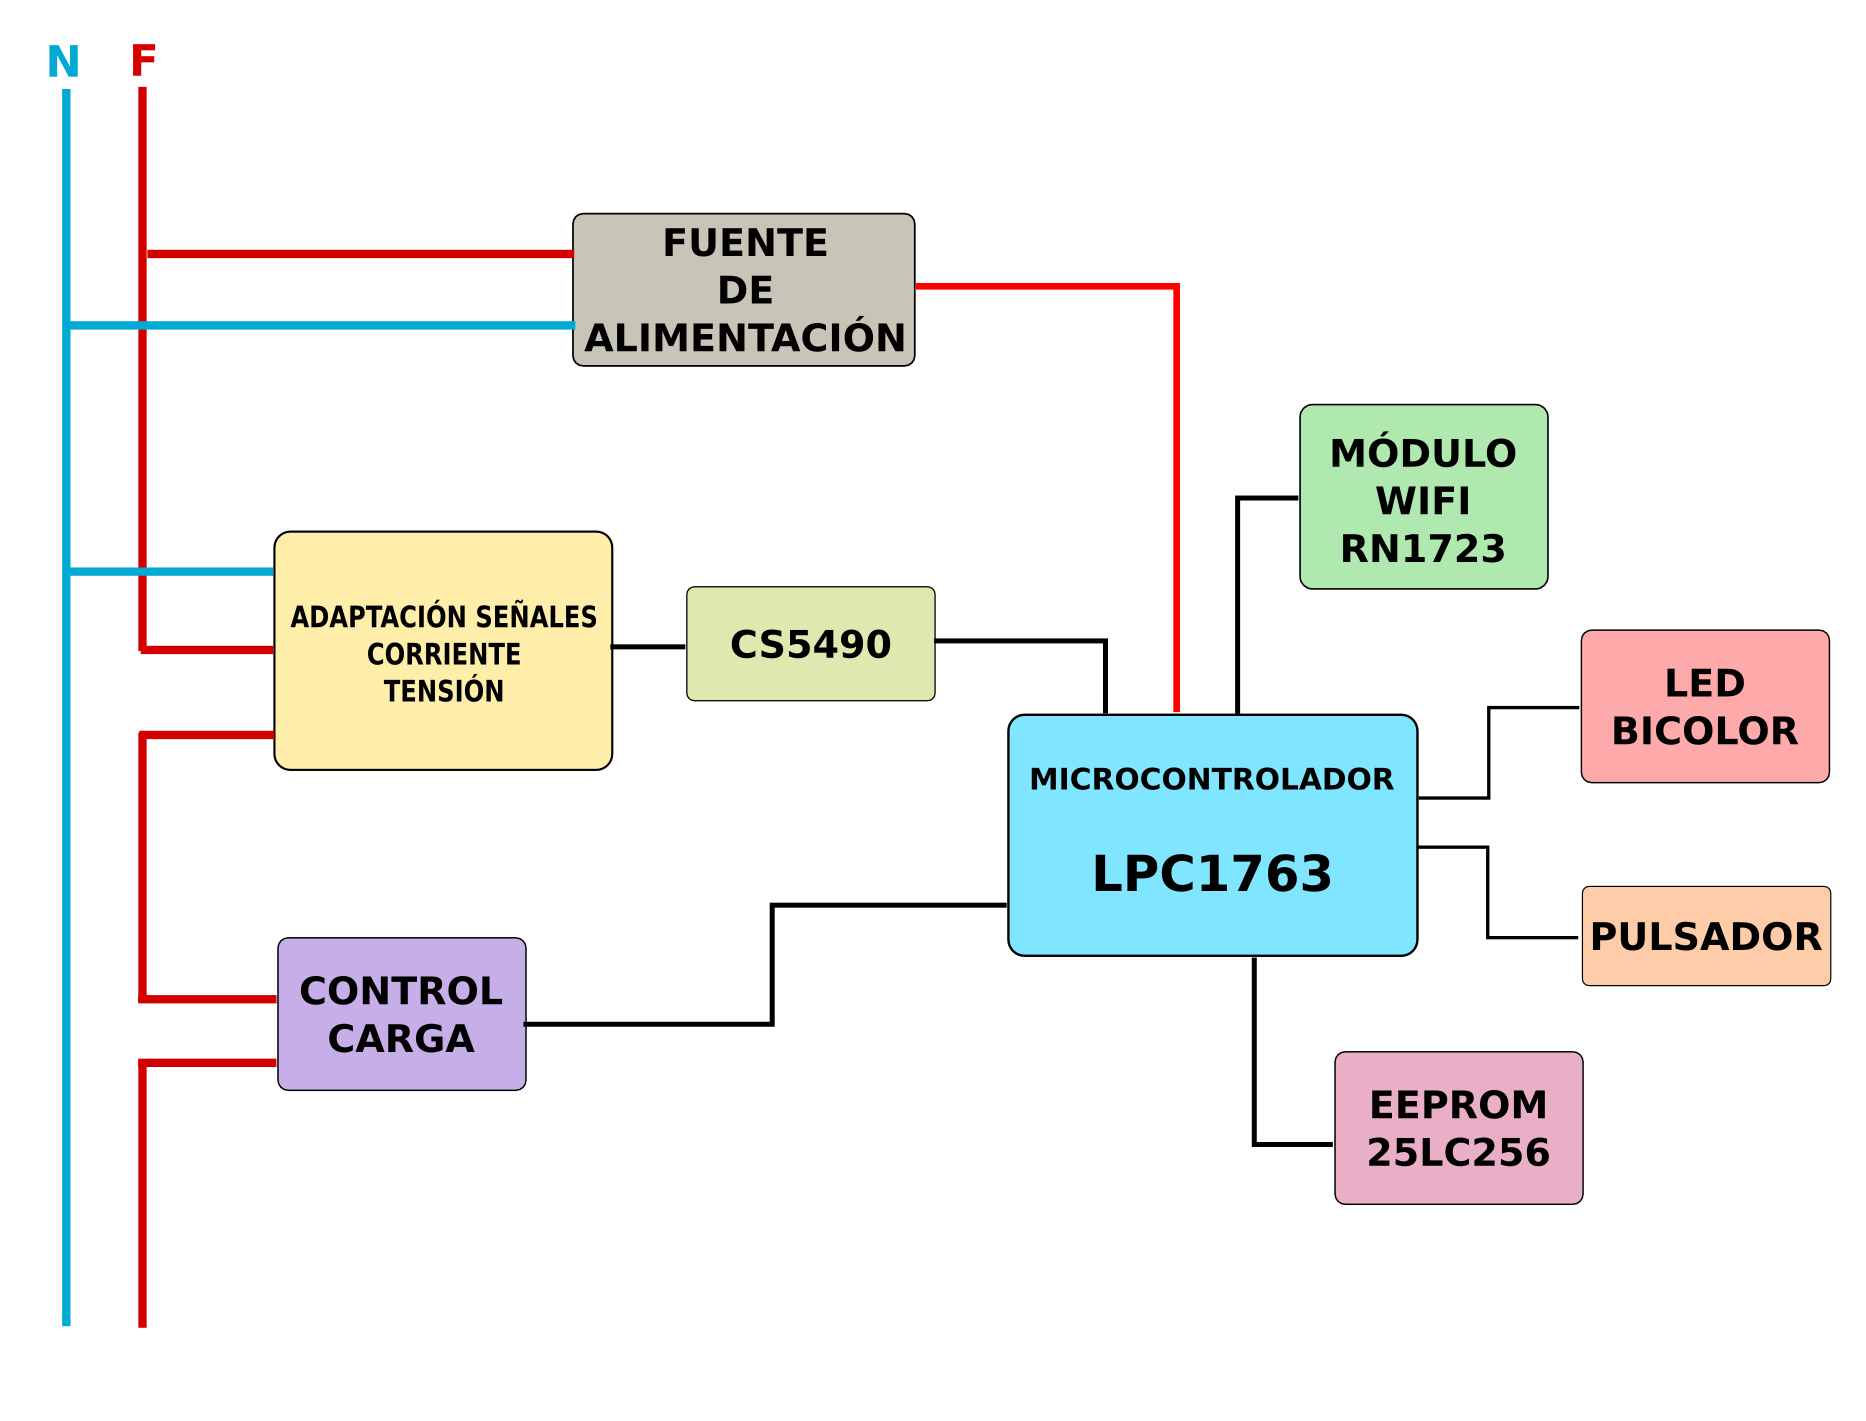
\includegraphics[width=12cm]{./Figures/3_1_1_diagrama_bloques_hardware.png}
	\caption{Diagrama en bloques del hardware del prototipo funcional.}
	\label{fig:hardware_diagrama_bloques}
\end{figure}

A continuación se describe brévemente cada uno de los módulos. Una explicación más detallada de cada uno se encuentra en la Subsección \ref{subsec:detalles_hardware}:

\begin{itemize}
\item Fuente de alimentación. La alimentación del equipo es obtenida de la misma línea eléctrica a la que está conectado el dispositivo. Debe generar dos niveles de tensión, 5V y 3,3V y debe ser capaz de entregar soportar el consumo especialmente del módulo WiFi.
\item Adaptación de las señales de corriente y tensión. Este bloque se encarga de adaptar la señal de tensión de la línea y la señal de la corriente consumida por el aparato eléctrico a los niveles que requiere el front-end analógico CS5490. La adaptación se realiza mediante transformadores para lograr una completa aislación de la línea.
\item Front-end analógico CS5490. Es el circuito integrado encargado de tomar las señales de la línea y generar las mediciones eléctricas de interés: tensión eficaz, corriente eficaz, frecuencia de línea, factor de potencia, energía consumida, etc.
\item Control de la carga. La conmutación de la carga se realiza mediante un relay mecánico.
\item Módulo WiFi RN1723. Es el módulo encargado de permitir la comunicación entre el Smart Plug y la aplicación móvil. Básicamente se encarga de esperar conexiones TCP y enviar las respuestas requeridas al socket del que provino el comando.
\item Microcontrolador LPC1763. Es el encargado de implementar la lógica del Smart Plug. 
\item Memoria EEPROM. Es la encargada de retener información de configuración del Smart Plug y las mediciones diarias de potencia y energía.
\item Led bicolor. Es un led rojo y verde encargado de realizar las señalizaciones acerca del funcionamiento del equipo. En la Subsección \ref{sec:validacion_firmware} se describe el significado de las distintas señalizaciones.
\item Pulsador. Mediante el pulsador se inician loas procesos destinados a incorporar el Smart Plug a la red WiFi de la casa.
\end{itemize}

\subsection{Descripción de los módulos de hardware}
\label{subsec:detalles_hardware}

En este apartado de la memoria se describen las decisiones de diseño asociadas a los módulos de hardware. Los fragmentos de esquemático que a continuación se muestran surgen del archivo \textit{SmartPlug\_v1.0} en \citep{repo_hardware}.

\subsubsection{Fuente de alimentación}

El esquemático de la fuente del Smart Plug puede verse en la Figura \ref{fig:pcb_fuente}. Esta fuente de alimentación se conecta a la misma línea eléctrica que es medida por el front-end analógico. A partir de la tensión de 220VAC genera una tensión de 5V y 3,3V. Para lograr los 5V se utiliza una fuente switching con montaje para PCB VSK-S2-5U la cual puede entregar hasta 400mA. Esta fuente permite generar una tensión estable manteniendo un empaquetado de reducido tamaño (34 x 22 x 18 mm). 

\begin{figure}[h]
	\centering
	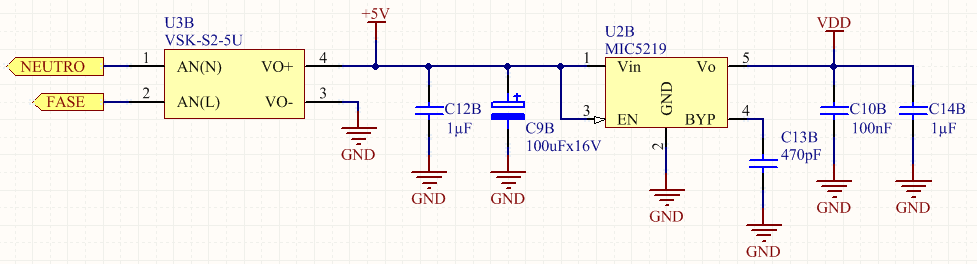
\includegraphics[width=14cm]{./Figures/3_1_2_pcb_fuente.png}
	\caption{Esquemático de la fuente de alimentación.}
	\label{fig:pcb_fuente}
\end{figure}


Se debe aclarar que esta switching fuente fue elegida para el prototipo funcional. En la versión final del equipo se utilizará una fuente switching AC-DC de similares características diseñada dentro de la empresa, debido a que tanto el tamaño del empaquetado de la fuente como su costo (U\$s 13,25 por unidad al momento de escribir la memoria) son prohibitivos para incluir esta fuente en el diseño final.

En cuanto al regular de 3,3V se eligió un componente que puede entrgar hasta 500mA. El requerimiento de corriente tanto de la fuente switching como del regulador de 3,3V surge del consumo especialmente del módulo WiFi RN1723, el cual puede consumir hasta 250mA.


\subsubsection{Adaptación de las señales de tensión y corriente}

En la Figura \ref{fig:pcb_adaptacion} puede verse la sección del esquemático relacionada con la adaptación de las señales de tensión y de corriente del dispositivo. Para poder obtener las mediciones eléctricas y el consumo de la carga conectada al Smart Plug es necesario adaptar las señales de tensión de línea y de la corriente consumida por la carga a los niveles soportados por el front-end analógico.

\begin{figure}[h]
	\centering
	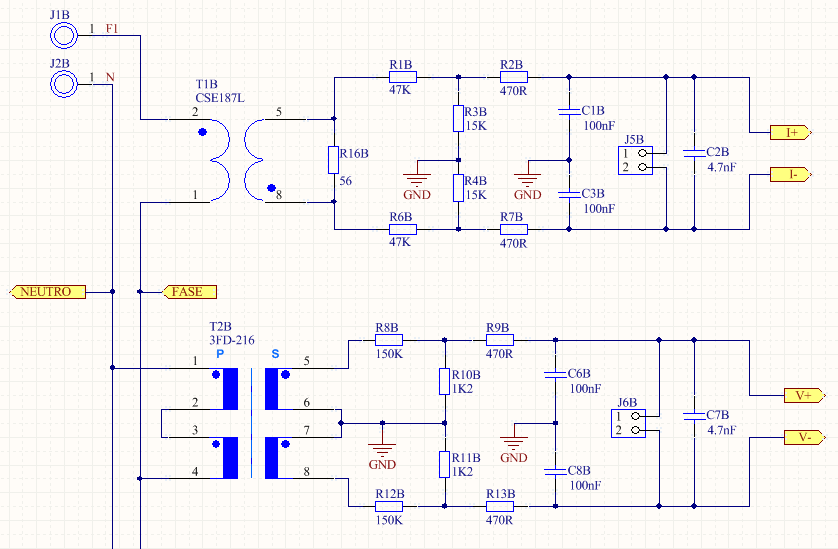
\includegraphics[width=14cm]{./Figures/3_1_2_pcb_adaptacion.png}
	\caption{Esquemático de la etapa de adaptación de las señales de tensión y corriente de la línea eléctrica.}
	\label{fig:pcb_adaptacion}
\end{figure}

De acuerdo a la hoja de datos del front-end elegido para este proyecto (CS5490) tanto la señal de corriente como la de tensión no deben superar los 250mV de pico en las entradas diferenciales del circuito integrado. Para lograr esto, primero se debe definir la tensión y la corriente máxima que debe medir el Smart Plug. En el caso concreto de este proyecto, y como ya fue mencionado, estos valores son: tensión máxima - 240VAC, corriente máxima - 5A.

Definidos estos valores, se eligió aislar el resto del circuito de la línea eléctrica tomando las señales de tensión y corriente mediante transformadores. Al igual que sucedió con la elección de la fuente switching, esta decisión fue exclusivamente para el desarrollo del prototipo funcional, ya que en la versión final será conveniente reemplazar el transformador de tensión por divisores resistivos y el transformador de corriente por un shunt. Ambos cambios van a permitir reducir el tamaño del producto final y su costo.

Luego de los transformadores hay divisores resistivos dispuestos en forma diferencial para reducir la tensión a los valores tolerados por el CS5409. Finalmente hay filtros pasa-bajo con un a frecuencia de corte de 3,3kHz.

Con los valores elegidos de relación de transformación y divisores resistivos, los valores máximos soportados por el equipo resultan:

\begin{itemize}
\item Tensión máxima soportada por el hardware: 320VAC.
\item Corriente máxima soportada por el hardware: 6,5A.
\end{itemize}

Ambos valores se encuentran por encima de los valores máximos informados al usuario.


\subsubsection{Front-end analógico}

Luego de adaptar las señales de tensión y de corriente, las mismas deben ser medidas por un front-end analógico que se encargará de generar los parámetros de interés para la aplicación: tensión y corriente eficaz, frecuencia de línea, potencia activa, factor de potencia, energía consumida, etc. En la Figura \ref{fig:pcb_medicion_energia} puede verse l circuito asociado al front-end elegido, el CS5490.

\begin{figure}[h]
	\centering
	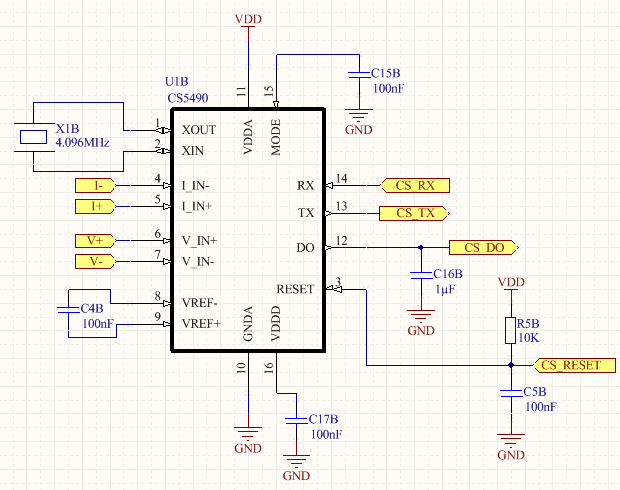
\includegraphics[width=14cm]{./Figures/3_1_2_pcb_medicion_energia.png}
	\caption{Esquemático del front-end analógico encargado de medir los parámetros eléctricos.}
	\label{fig:pcb_medicion_energia}
\end{figure}

A parte de los componentes relacionados con la adaptación de las señales de línea, este circuito integrado  no necesita de una gran cantidad de componentes adicionales, salvo algunos capacitores y un cristal de 4,096Mhz con el cual va generar la base de tiempo interna para realizar las mediciones y cálculos.

La comunicación es sencilla, a través de comandos enviados por una UART. Con estos comandos se van poder conocer casi todas las mediciones que calcula el CS5490. La única medición que no puede ser conocida a través de la lectura de un registro es la energía consumida. Esta es informada mediante pulsos a través del pin \textit{DO}. Se debe configurar la constante del medidor en el CS5490, es decir la cantidad de pulsos a los que equivale un kilowatt-hora.


\subsubsection{Control de la carga}

La conmutación de la carga está a cargo de un relay mecánico. En la Figura \ref{fig:pcb_control_carga} puede verse que la fase de la línea eléctrica se conecta entre los contactos \textit{común} y \textit{normal cerrado} del relay para que, en caso de ocurrir un desperfecto con el Smart Plug, la carga pueda seguir funcionando.

\begin{figure}[h]
	\centering
	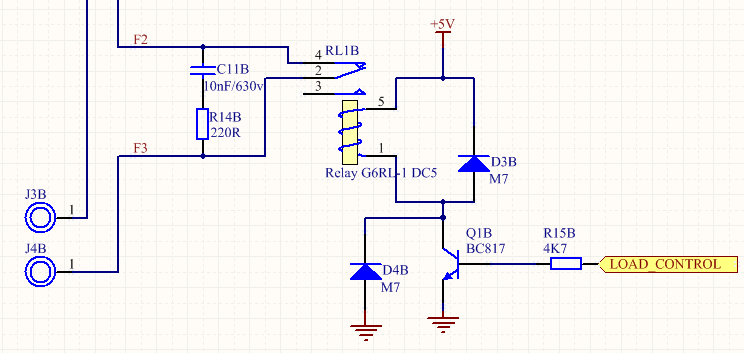
\includegraphics[width=10cm]{./Figures/3_1_2_pcb_control_carga.png}
	\caption{Esquemático del control de la carga eléctrica mediante un relay mecánico.}
	\label{fig:pcb_control_carga}
\end{figure}

Para funcionar, la bobina del relay requiere de una tensión de 5V y los contactos soportan una corriente máxima de 8A con 250VAC, valor que satisface sobradamente las especificaciones propuestas para el Smart Plug.

\subsubsection{Módulo WiFi}

En la Figura \ref{fig:pcb_wifi} se muestra el esquemático asociado al módulo WiFi. El módulo elegido es el RN1723, el cual prácticamente no requiere de componentes adicionales y se comunica con el microcontrolador mediante una UART.

\begin{figure}[h]
	\centering
	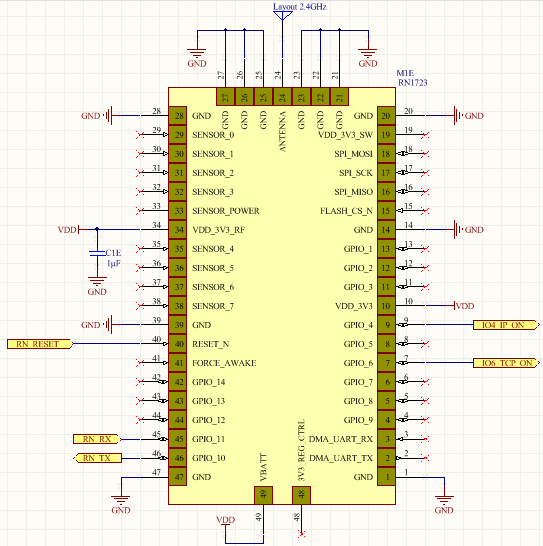
\includegraphics[width=12cm]{./Figures/3_1_2_pcb_wifi.png}
	\caption{Esquemático del módulo WiFi.}
	\label{fig:pcb_wifi}
\end{figure}

Para la antena del módulo se eligió una antena impresa en el PCB de acuerdo a las especificaciones de la hoja de datos del módulo.

Al momento de comenzar con el proyecto y elegir los componentes, este módulo resultaba una opción atractiva, que proveía las funcionalidades especificadas en los requerimientos del producto a un precio aceptable. Además se decidió elegir este módulo ya que es comercializado por Microchip, marca que es ampliamente usada por los productos de X-28 Alarmas, lo cual lleva a la posibilidad de obtener precios muy competitivos con los distribuidores.

\section{Firmware}

\subsection{Arquitectura del firmware}

\begin{figure}[h]
	\centering
	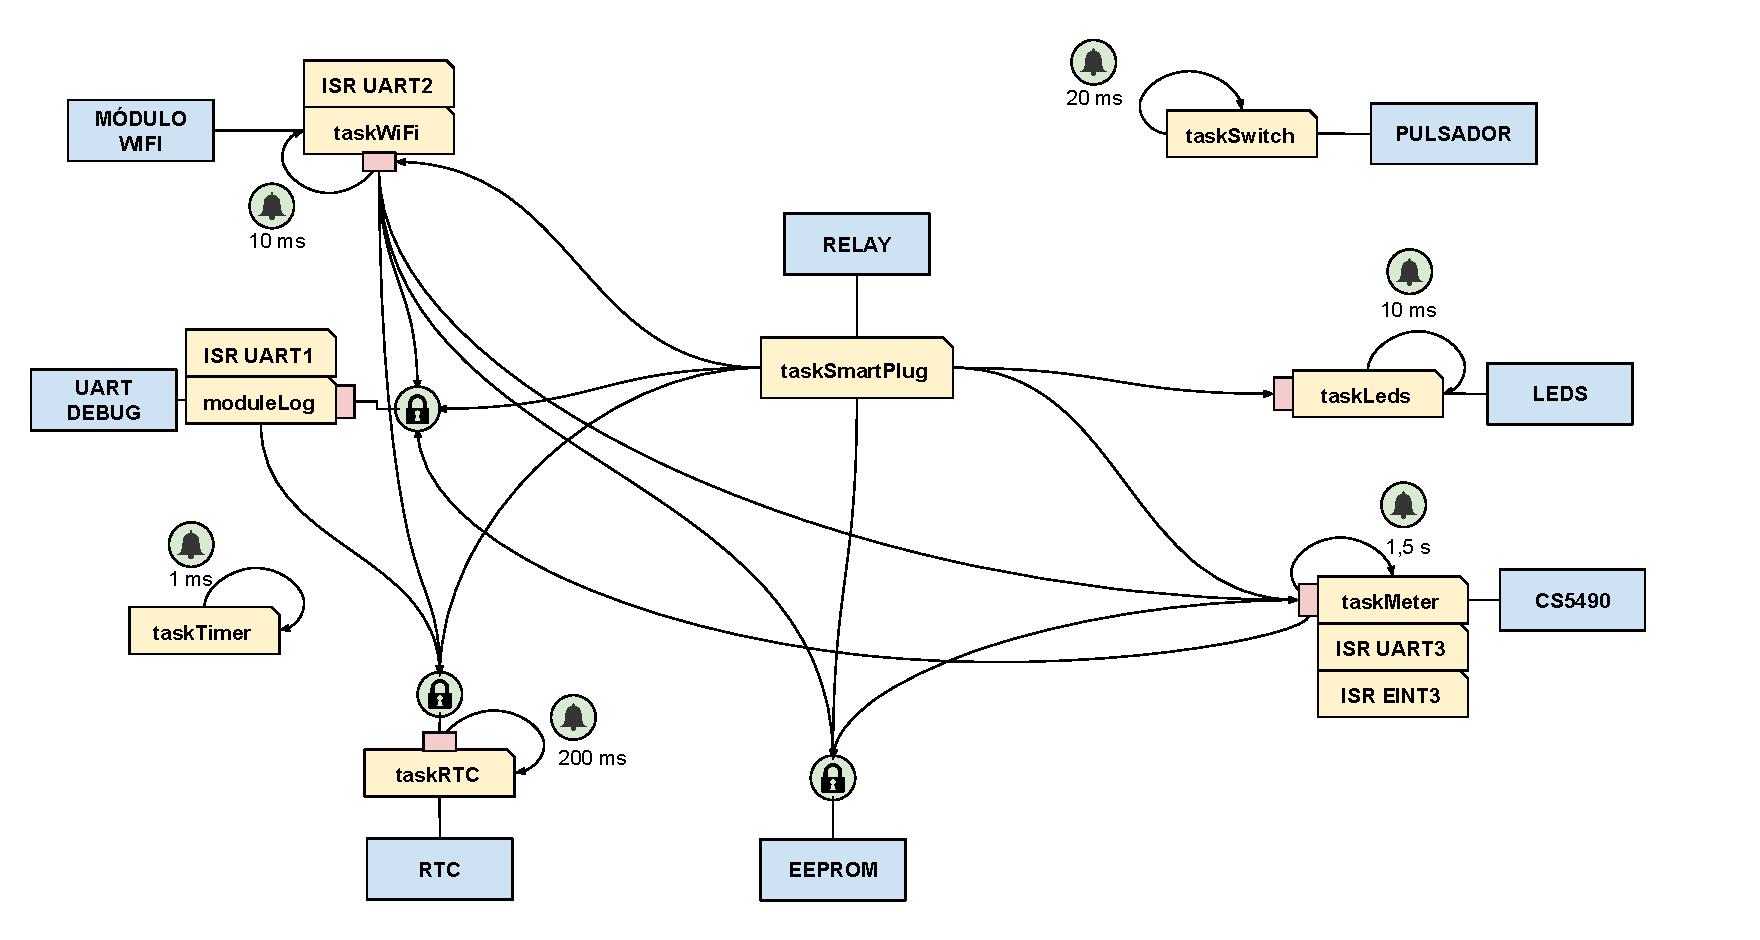
\includegraphics[width=16cm]{./Figures/3_2_1_firmware_esquema_tareas.pdf}
	\caption{Esquema de las tareas y recursos utilizados en el firmware.}
	\label{fig:firmware_esquema_tareas}
\end{figure}


\subsection{Capas de abstracción}

\begin{figure}[h]
	\centering
	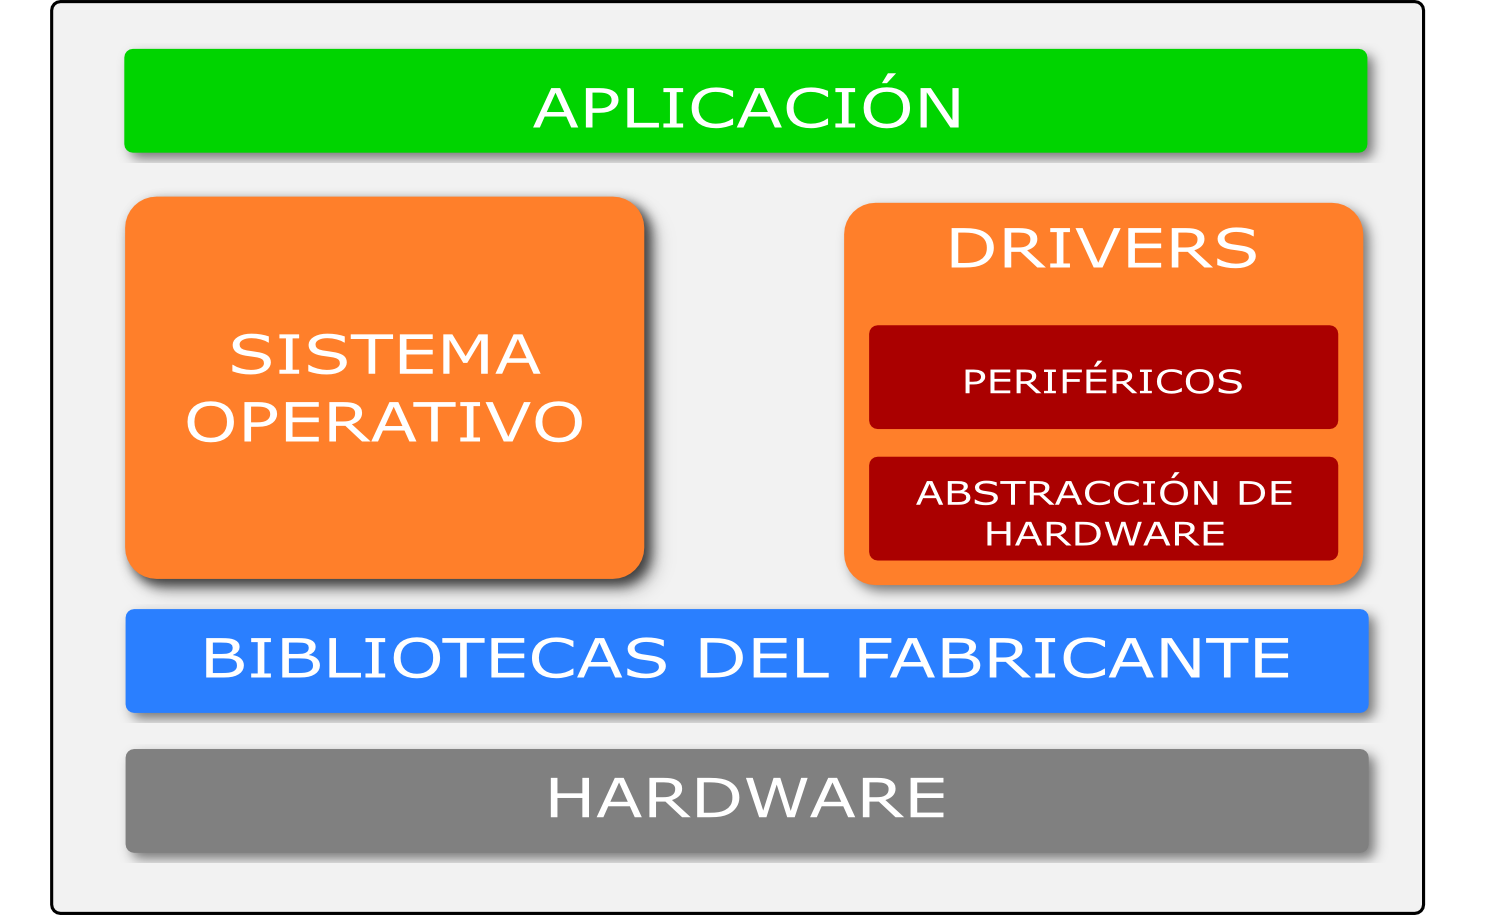
\includegraphics[width=10cm]{./Figures/3_2_2_firmware_diagrama_capas.png}
	\caption{Capas del firmware.}
	\label{fig:firmware_diagrama_capas}
\end{figure}


\subsection{Metodología orientada a objetos}

\begin{figure}[h]
	\centering
	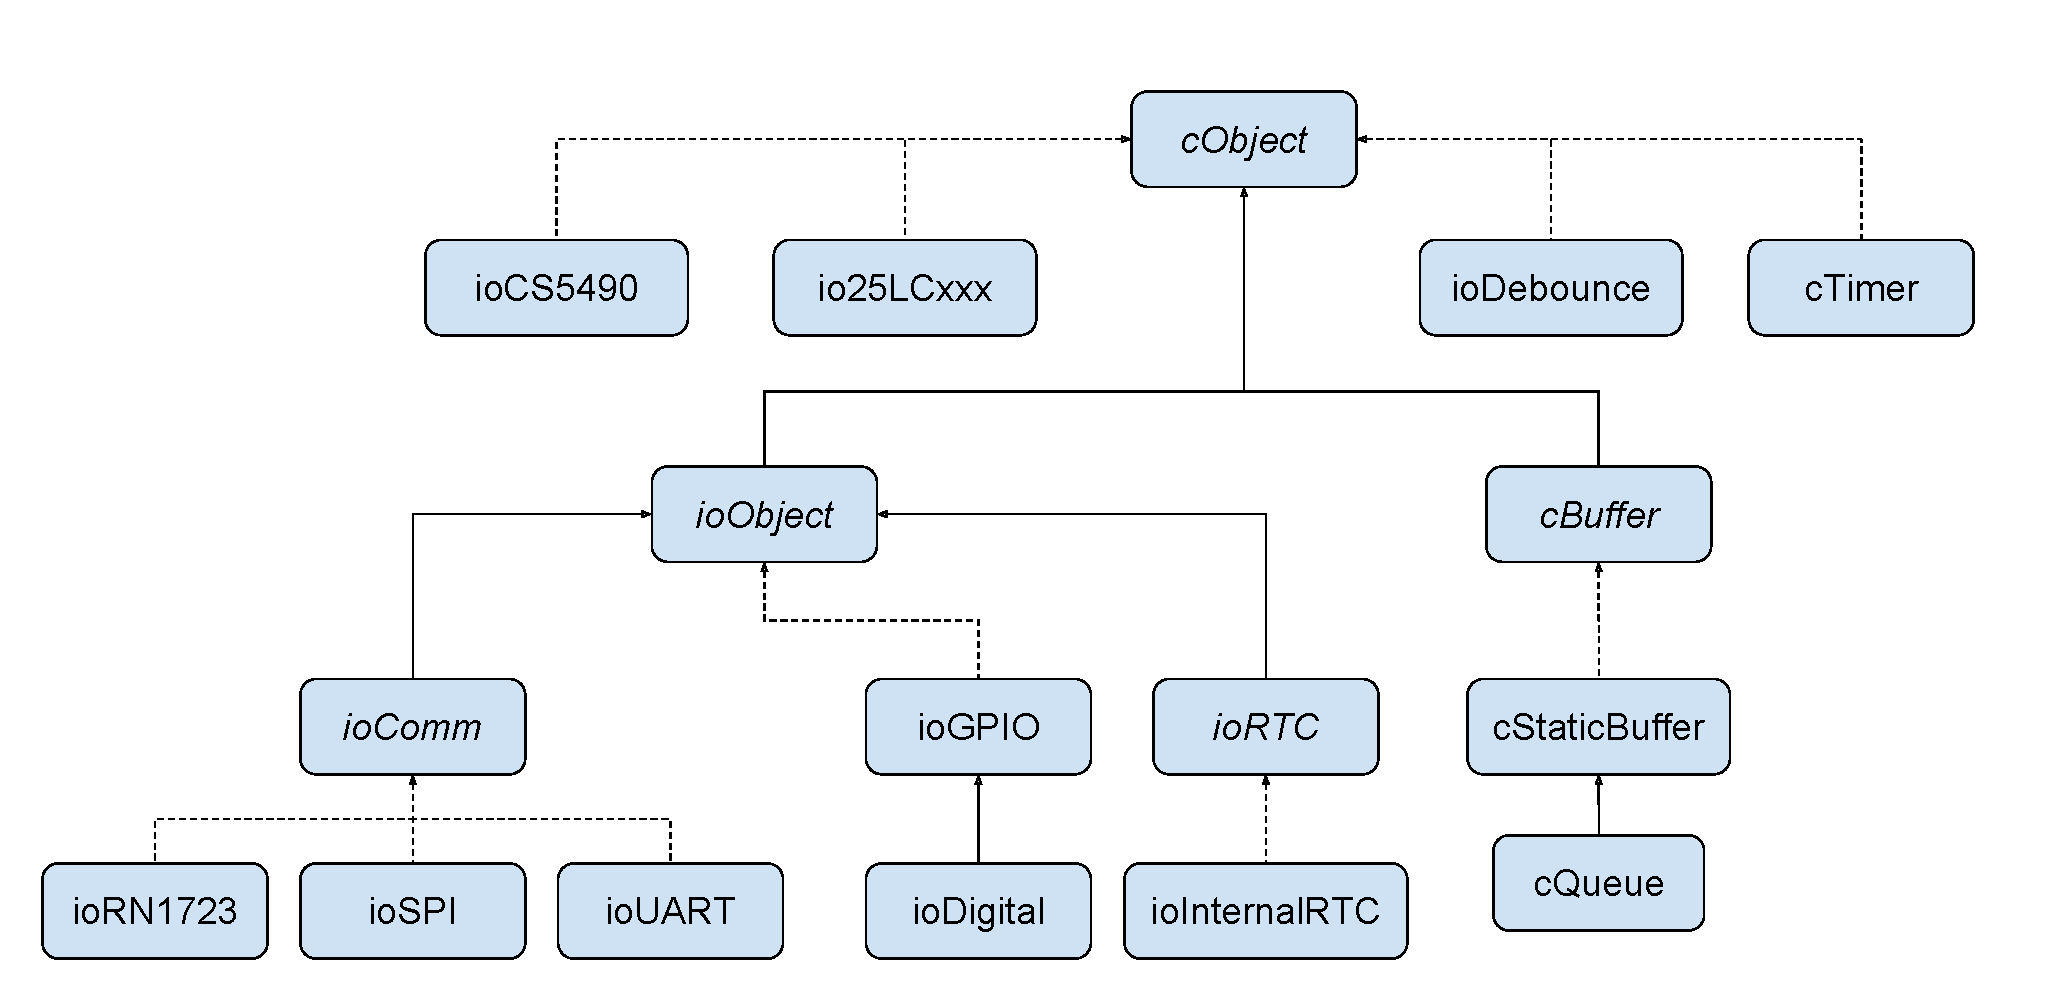
\includegraphics[width=14cm]{./Figures/3_2_3_diagrama-clases-simplificado.pdf}
	\caption{Diagrama de clases de los controladores desarrollados para el firmware.}
	\label{fig:firmware_diagrama_clases}
\end{figure}


\subsection{Protocolo de comunicación}
\label{subsection:protocolo}

\begin{figure}[h]
	\centering
	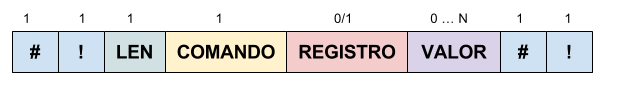
\includegraphics[width=12cm]{./Figures/3_2_4_formato_trama.png}
	\caption{Formato de la trama.}
	\label{fig:formato_trama}
\end{figure}


\subsection{Uso de los comandos}

\begin{figure}[h]
	\centering
	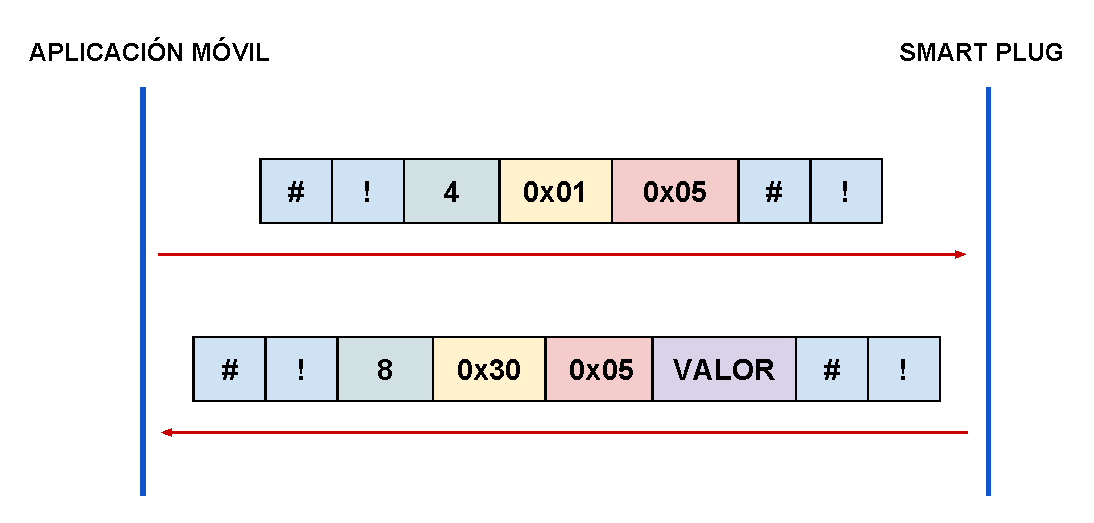
\includegraphics[width=12cm]{./Figures/3_2_5_comunicacion_GET.pdf}
	\caption{Diagrama de comunicación del comando \textit{GET}.}
	\label{fig:comunicacion_get}
\end{figure}


\begin{figure}[h]
	\centering
	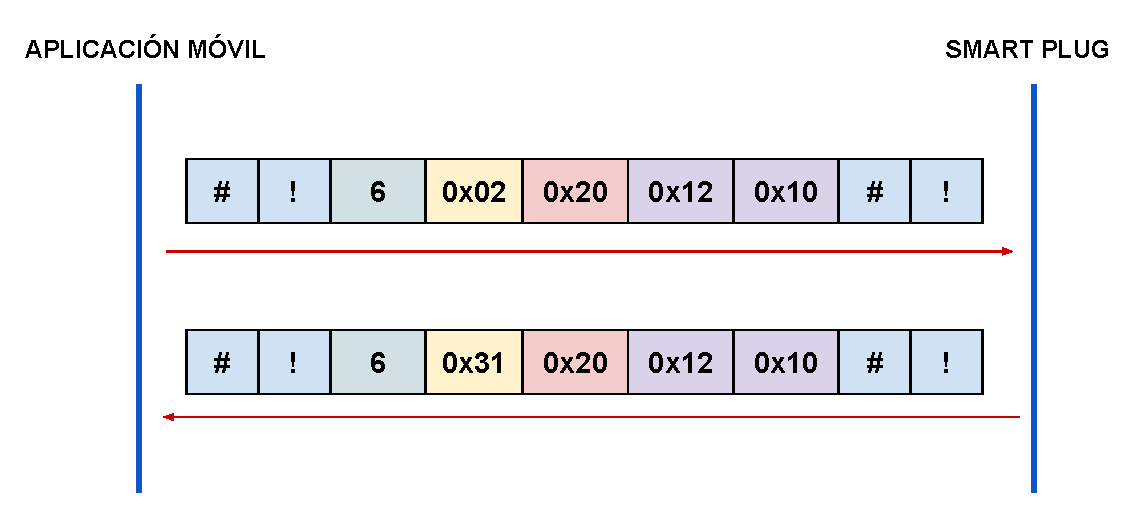
\includegraphics[width=12cm]{./Figures/3_2_5_comunicacion_SET.pdf}
	\caption{Diagrama de comunicación del comando \textit{SET}.}
	\label{fig:comunicacion_set}
\end{figure}


\begin{figure}[h]
	\centering
	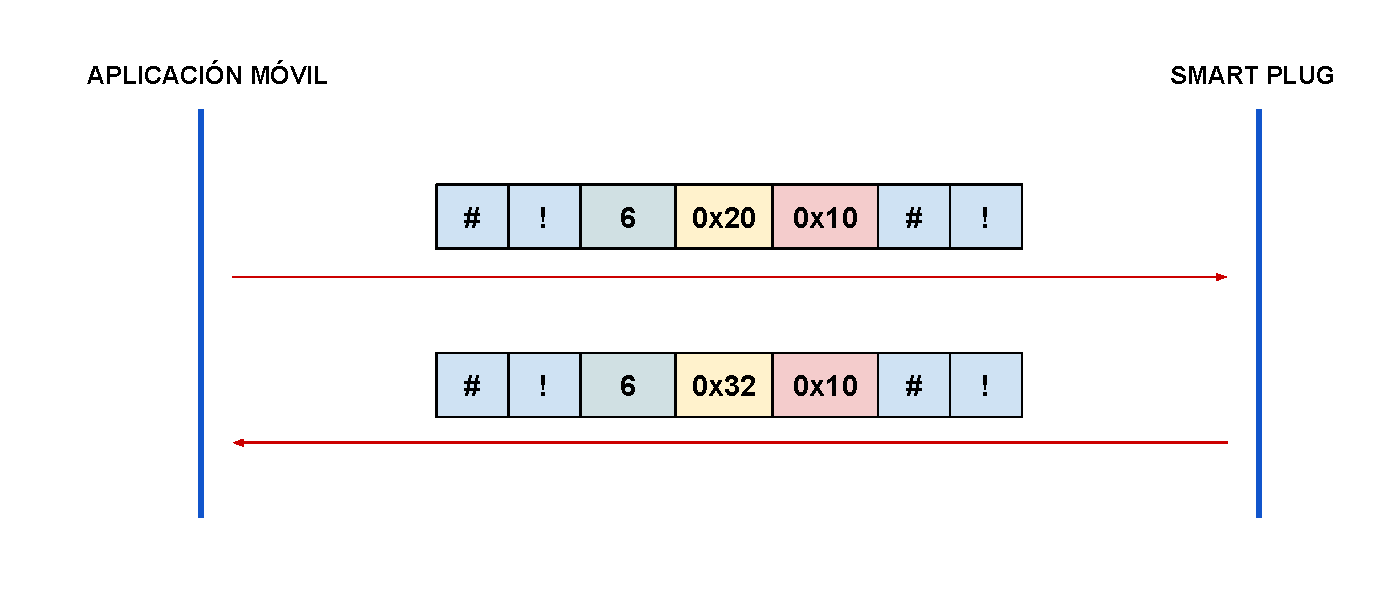
\includegraphics[width=12cm]{./Figures/3_2_5_comunicacion_RESET.pdf}
	\caption{Diagrama de comunicación del comando \textit{RESET}.}
	\label{fig:comunicacion_reset}
\end{figure}


\begin{figure}[h]
	\centering
	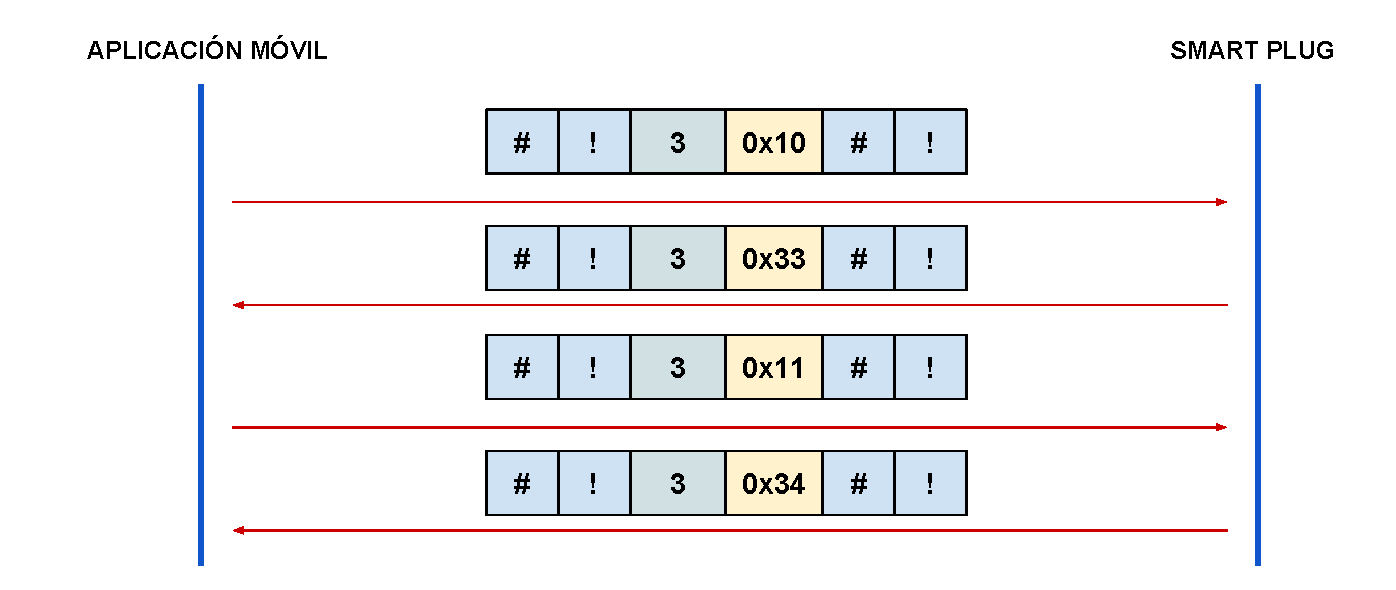
\includegraphics[width=12cm]{./Figures/3_2_5_comunicacion_NODE.pdf}
	\caption{Diagrama de comunicación de los comandos \textit{NODE ON} y \textit{NODE OFF}.}
	\label{fig:comunicacion_node}
\end{figure}


\section{Aplicación Android}
\label{section:app}

\subsection{Maqueta de la aplicación}

\begin{figure}[h]
	\centering
	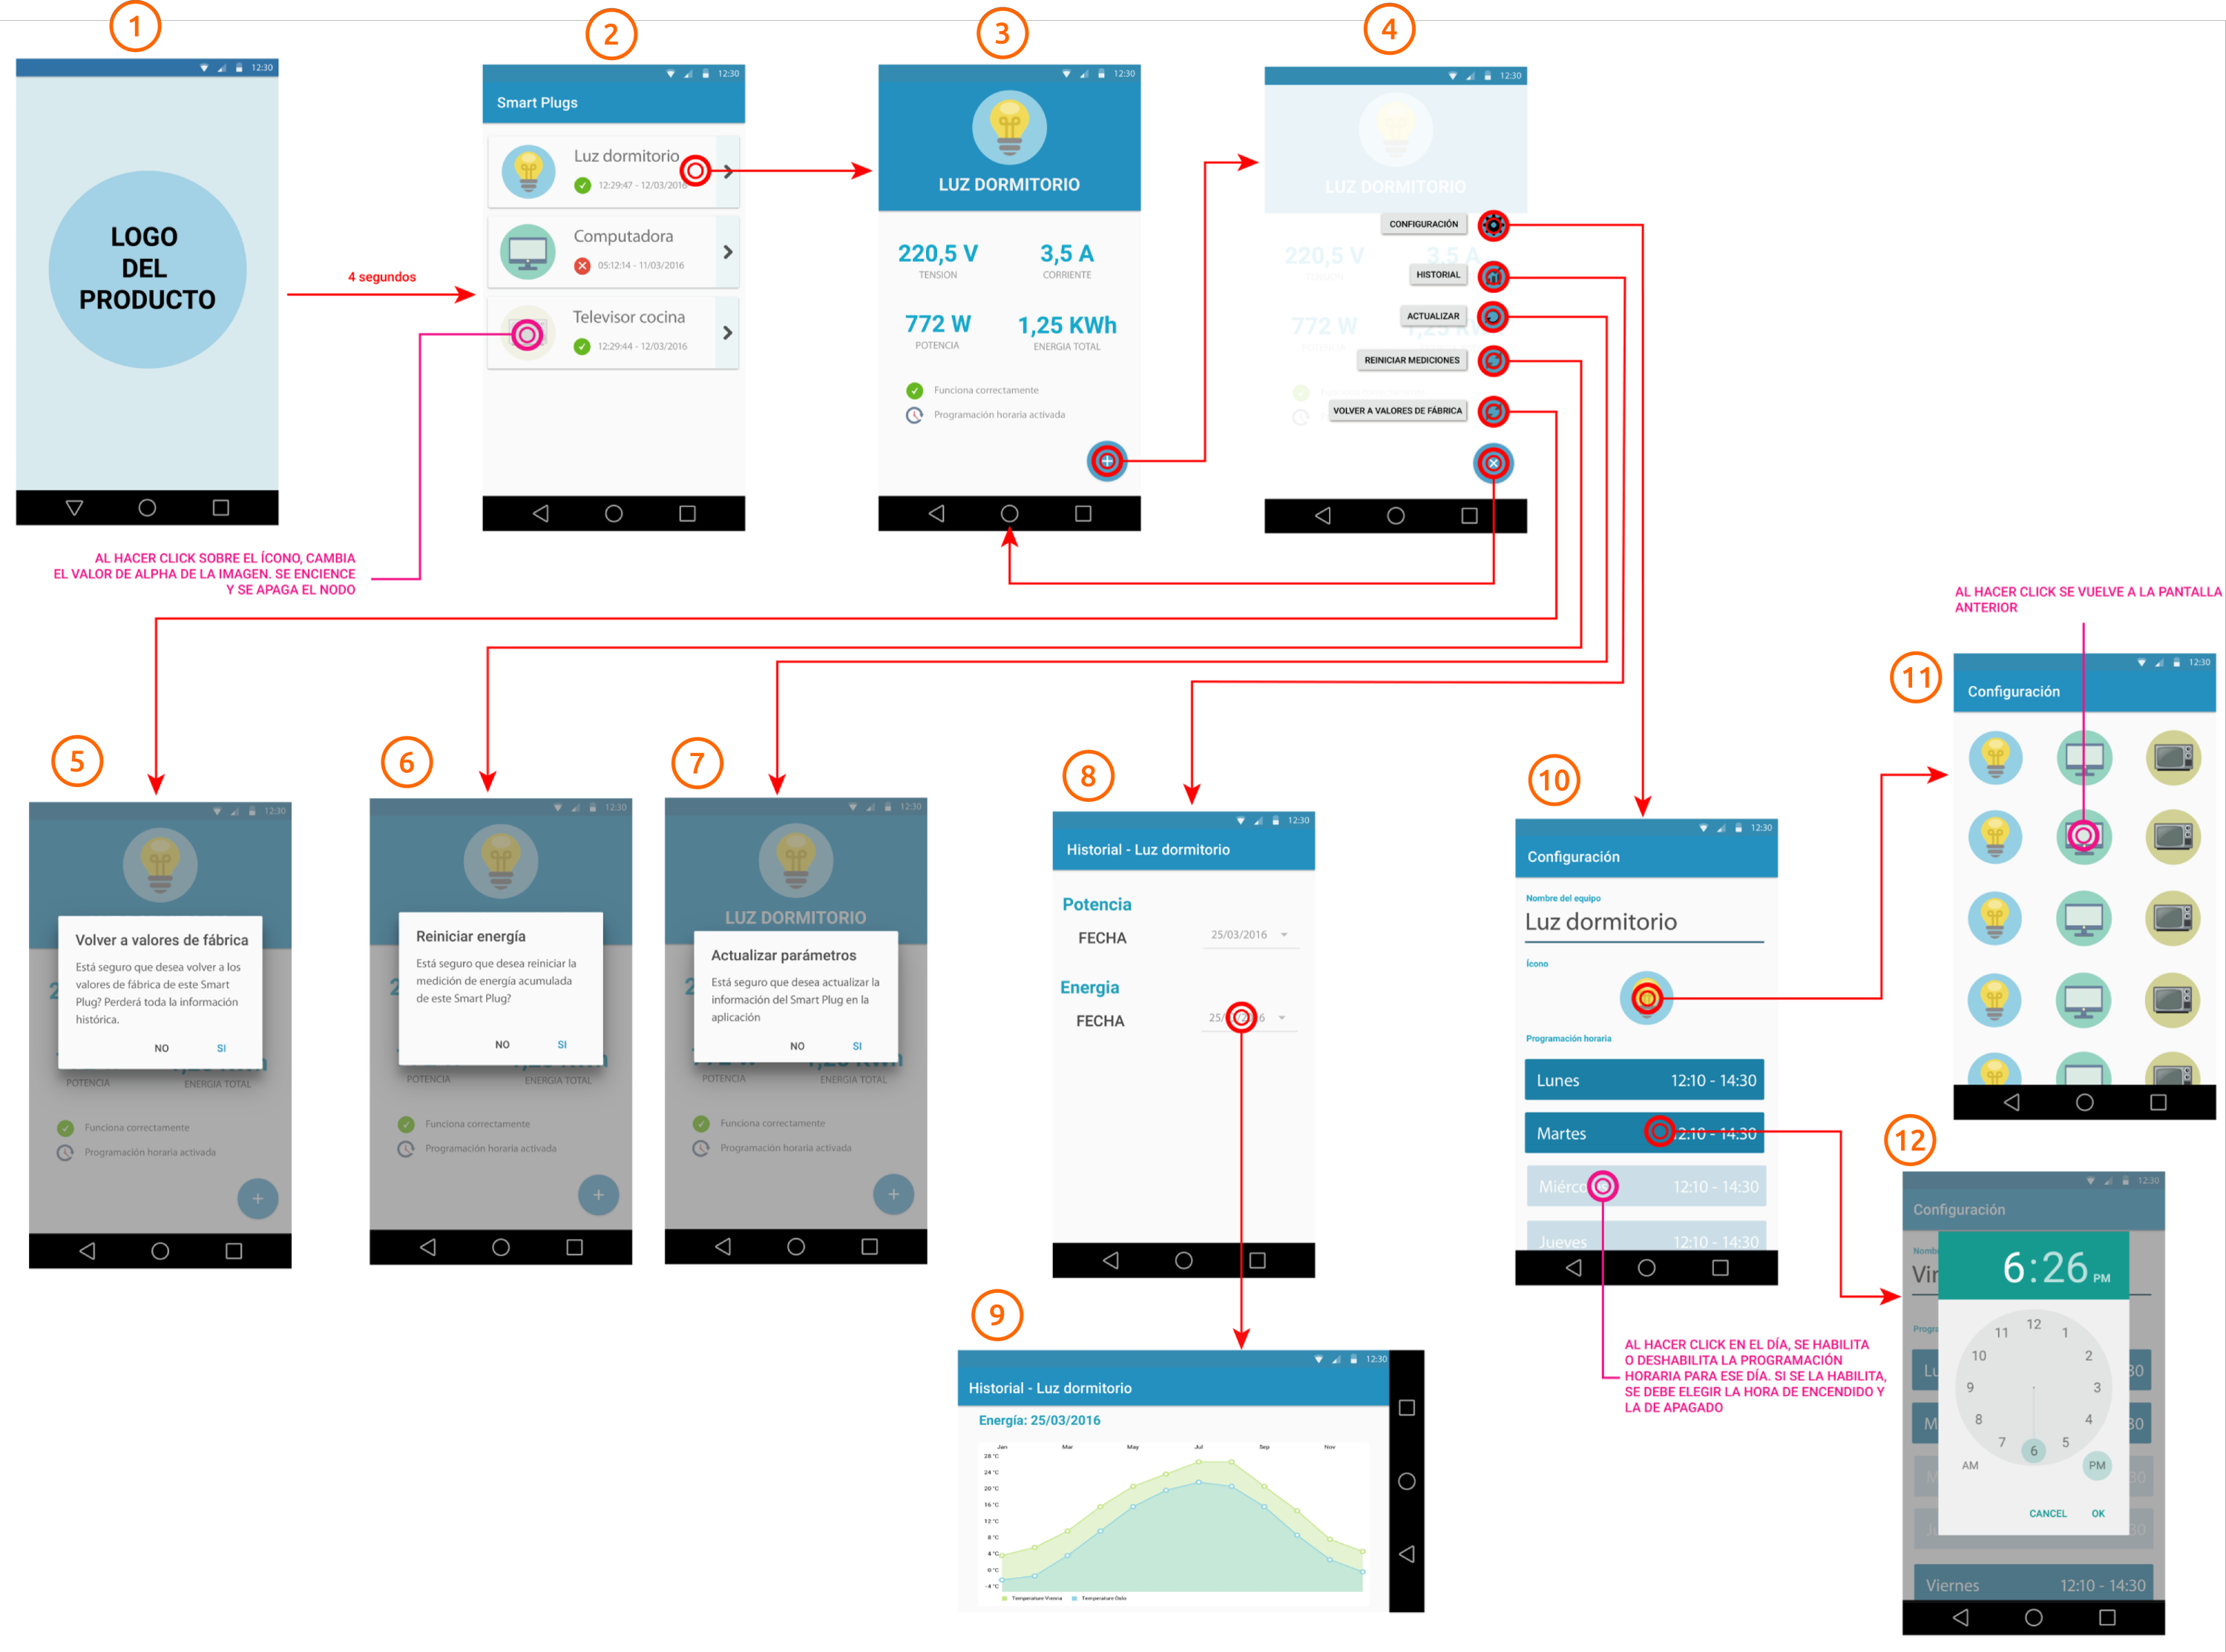
\includegraphics[width=18cm, angle=90]{./Figures/3_3_1_app_wireframe.png}
	\caption{Maqueta de la aplicación móvil.}
	\label{fig:comunicacion_app_wireframe}
\end{figure}


\subsection{Arquitectura de la aplicación}

\begin{figure}[h]
	\centering
	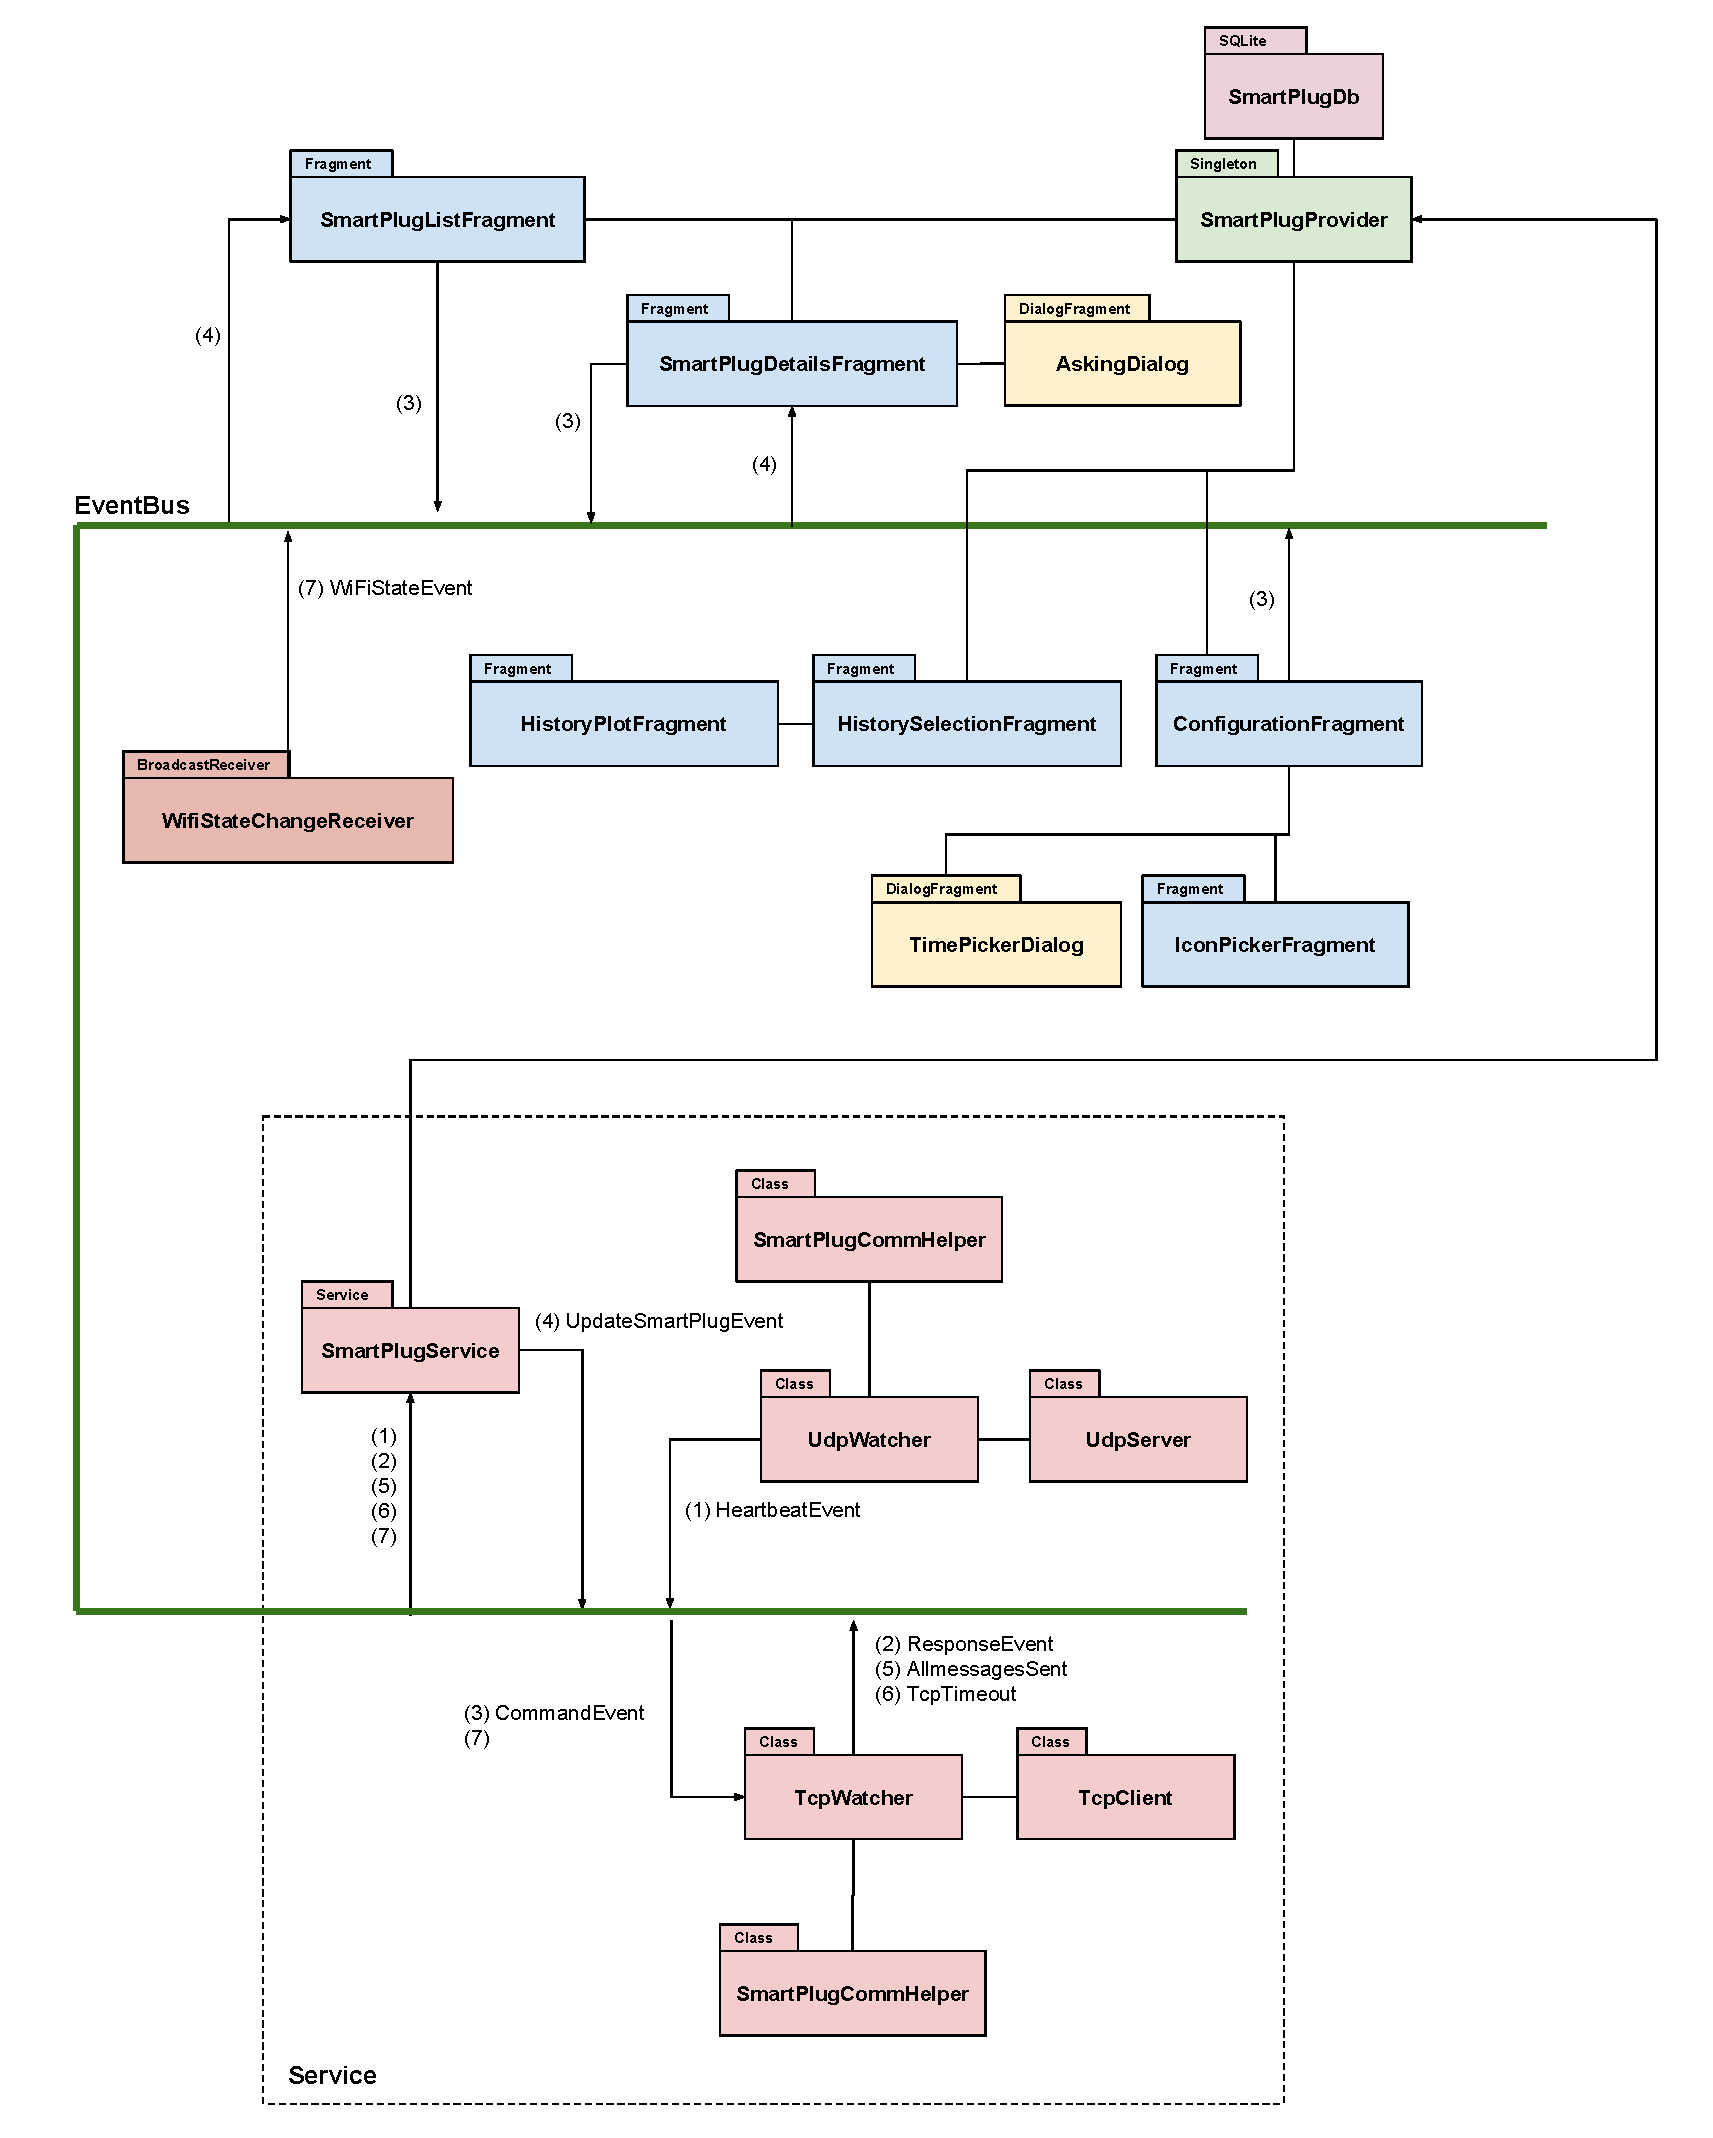
\includegraphics[width=14cm]{./Figures/3_3_2_app-arquitectura.pdf}
	\caption{Relación entre las clases desarrolladas para la aplicación móvil.}
	\label{fig:app_arquitectura}
\end{figure}



